\documentclass[11pt, a4paper]{article}

% Fonts and Encoding
\usepackage[utf8]{inputenc}
\usepackage[T1]{fontenc}

% Math and Symbols
\usepackage{amsmath, amssymb, amsthm, amsfonts, mathrsfs, mathtools}

% Layout and Geometry
\usepackage{geometry}
\geometry{a4paper, margin=1in}

% Formatting and Graphics
\usepackage{graphicx, xcolor, enumitem, booktabs, array, tabularx}

% TikZ for Illustrations
\usepackage{tikz}
\usetikzlibrary{arrows.meta, positioning, shapes.geometric, calc, backgrounds, matrix}

% Clickable Links and TOC
\usepackage{hyperref}
\hypersetup{
    colorlinks=true,
    linkcolor=blue,
    filecolor=magenta,      
    urlcolor=cyan,
    pdftitle={Advanced Mathematics Topic},
}

% Theorem Environments
\newtheorem{theorem}{Theorem}[section]
\newtheorem{lemma}[theorem]{Lemma}
\newtheorem{proposition}[theorem]{Proposition}
\newtheorem{corollary}[theorem]{Corollary}
\theoremstyle{definition}
\newtheorem{definition}{Definition}[section]
\newtheorem{axiom}{Axiom}[section]
\newtheorem{example}{Example}[section]
\theoremstyle{remark}
\newtheorem{remark}{Remark}[section]

% Custom Commands (Enforced standard notation)
\newcommand{\R}{\mathbb{R}}
\newcommand{\N}{\mathbb{N}}
\newcommand{\Z}{\mathbb{Z}}
\newcommand{\Q}{\mathbb{Q}}
\newcommand{\E}{\mathbb{E}}
\newcommand{\Prob}{\mathbb{P}}
\newcommand{\F}{\mathcal{F}}

\title{\textbf{Comprehensive Study Guide: The Annihilator Method and Undetermined Coefficients}}
\author{Tashfeen Omran}
\date{October 29, 2026}

\begin{document}

\maketitle
\tableofcontents
\newpage

\section{Comprehensive Introduction, Context, and Prerequisites}

\subsection{Core Concepts and Intuition}
The study of linear differential equations is a cornerstone of applied mathematics. A linear differential equation with constant coefficients takes the form:
\[
a_n y^{(n)} + a_{n-1} y^{(n-1)} + \dots + a_1 y' + a_0 y = g(x)
\]
When $g(x) = 0$, the equation is called \textbf{homogeneous}. When $g(x) \neq 0$, it is \textbf{nonhomogeneous}. The general solution to a nonhomogeneous equation is always the sum of two parts:
\[
y(x) = y_c(x) + y_p(x)
\]
where $y_c(x)$ is the \textit{complementary solution} (the general solution to the associated homogeneous equation) and $y_p(x)$ is a \textit{particular solution} (any single solution that satisfies the nonhomogeneous equation).

The \textbf{Method of Undetermined Coefficients} is a technique for finding $y_p(x)$ when $g(x)$ consists of polynomials, exponentials, sines, cosines, or finite sums and products of these. The intuition is simple: since taking derivatives of these functions yields functions of the same type, we can "guess" that $y_p(x)$ has the same form as $g(x)$, but with unknown coefficients. We then substitute this guess into the differential equation to determine the coefficients.

However, guessing can be tricky, especially when the terms in $g(x)$ overlap with the terms in $y_c(x)$. To eliminate the guesswork, we use the \textbf{Annihilator Method}. 

\subsection{The Annihilator Method}
We introduce the differential operator $D = \frac{d}{dx}$. A polynomial in $D$, denoted $P(D)$, can be applied to a function $y$. For example, $(D^2 - 3D + 2)y = y'' - 3y' + 2y$.

An \textbf{annihilator} of a function $g(x)$ is a differential operator $A(D)$ such that:
\[
A(D)[g(x)] = 0
\]
By applying $A(D)$ to both sides of the nonhomogeneous equation $P(D)y = g(x)$, we obtain a new, higher-order \textit{homogeneous} equation:
\[
A(D)P(D)y = 0
\]
Solving this new homogeneous equation gives us the exact structural form of $y_p(x)$, completely removing the need for ad-hoc guessing.

\begin{center}
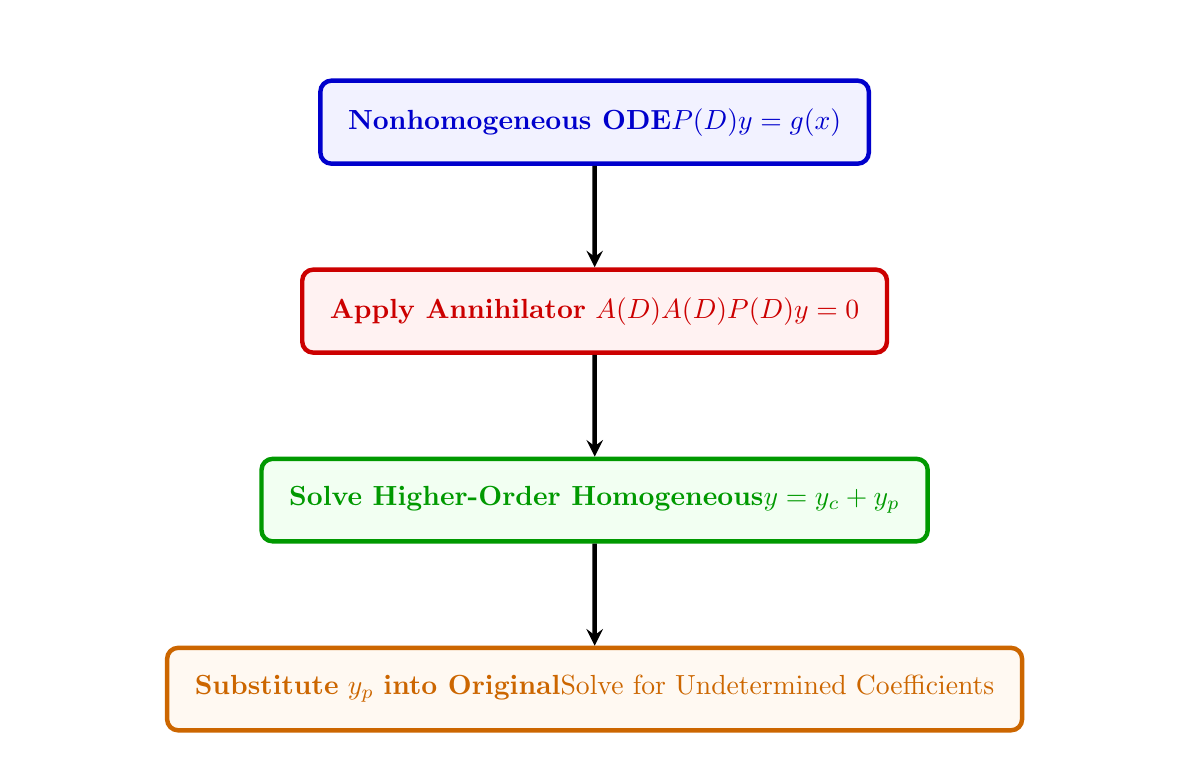
\begin{tikzpicture}[scale=1.2]
    % Background fill to ensure safe rendering
    \fill[white] (-2,-1) rectangle (10, 6);
    
    % Nodes
    \node[draw, ultra thick, blue!80!black, rounded corners, inner sep=10pt, fill=blue!5] (ode) at (4, 5) {\textbf{Nonhomogeneous ODE} \\ $\displaystyle P(D)y = g(x)$};
    
    \node[draw, ultra thick, red!80!black, rounded corners, inner sep=10pt, fill=red!5] (ann) at (4, 3) {\textbf{Apply Annihilator} $A(D)$ \\ $\displaystyle A(D)P(D)y = 0$};
    
    \node[draw, ultra thick, green!60!black, rounded corners, inner sep=10pt, fill=green!5] (hom) at (4, 1) {\textbf{Solve Higher-Order Homogeneous} \\ $\displaystyle y = y_c + y_p$};
    
    \node[draw, ultra thick, orange!80!black, rounded corners, inner sep=10pt, fill=orange!5] (sub) at (4, -1) {\textbf{Substitute} $y_p$ \textbf{into Original} \\ \text{Solve for Undetermined Coefficients}};
    
    % Arrows
    \draw[->, >=stealth, ultra thick] (ode) -- (ann);
    \draw[->, >=stealth, ultra thick] (ann) -- (hom);
    \draw[->, >=stealth, ultra thick] (hom) -- (sub);
\end{tikzpicture}
\end{center}

\subsection{Historical Context and Motivation}
In the 18th and 19th centuries, mathematicians like Leonhard Euler and Joseph-Louis Lagrange were studying the motion of planets, vibrating strings, and pendulums. These physical systems are often subjected to external forces (like a periodic push on a pendulum). The homogeneous equation models the system's natural, unforced behavior, while the nonhomogeneous term $g(x)$ models the external forcing. The Method of Undetermined Coefficients was developed to find the system's specific response to these external forces.

\subsection{Prerequisites}
To master this topic, you must be proficient in:
\begin{itemize}
    \item \textbf{Factoring Polynomials:} Finding roots of characteristic equations, including complex roots.
    \item \textbf{Solving Homogeneous Linear ODEs:} Knowing how roots of the characteristic equation translate into solutions (e.g., real roots, repeated roots, complex conjugate roots).
    \item \textbf{Differentiation Rules:} Product rule, chain rule, and higher-order derivatives.
\end{itemize}

\newpage
\section{Detailed Homework Solutions}

\subsection*{Problem 1}
\textbf{Statement:} Use the method of undetermined coefficients to determine the form of a particular solution for the given equation:
\[
y''' + 10y'' - 11y = xe^x + 12x
\]

\textbf{Solution:}
First, we find the complementary solution $y_c(x)$ by solving the homogeneous equation $y''' + 10y'' - 11y = 0$. The characteristic equation is:
\[
r^3 + 10r^2 - 11 = 0
\]
By inspection, $r = 1$ is a root since $1 + 10 - 11 = 0$. We can factor the polynomial using synthetic division or algebraic manipulation:
\[
r^3 - r^2 + 11r^2 - 11r + 11r - 11 = r^2(r-1) + 11r(r-1) + 11(r-1) = (r-1)(r^2 + 11r + 11) = 0
\]
The roots are $r_1 = 1$ and $r_{2,3} = \frac{-11 \pm \sqrt{121 - 44}}{2} = \frac{-11 \pm \sqrt{77}}{2}$. 
Thus, the complementary solution contains $e^x$.

Next, we analyze the nonhomogeneous term $g(x) = xe^x + 12x$.
\begin{itemize}
    \item The term $xe^x$ is annihilated by $(D-1)^2$.
    \item The term $12x$ is annihilated by $D^2$.
\end{itemize}
The total annihilator is $A(D) = D^2(D-1)^2$. Applying this to the ODE gives a new characteristic equation:
\[
r^2(r-1)^2 (r-1)(r^2 + 11r + 11) = 0 \implies r^2(r-1)^3(r^2 + 11r + 11) = 0
\]
The roots of this new equation dictate the form of the general solution:
\[
y(x) = \underbrace{c_1 e^x + c_2 e^{r_2 x} + c_3 e^{r_3 x}}_{y_c(x)} + \underbrace{c_4 x e^x + c_5 x^2 e^x + c_6 + c_7 x}_{y_p(x)}
\]
Renaming the constants for the particular solution, we get:
\[
y_p(x) = (Ax^2 + Bx)e^x + Cx + F
\]
\textbf{Final Answer:} $y_p(x) = (Ax^2 + Bx)e^x + Cx + F$

\vspace{1em}
\subsection*{Problem 2}
\textbf{Statement:} Find a general solution to the given equation:
\[
y''' - 6y'' + 12y' - 8y = 2e^{2x}
\]

\textbf{Solution:}
The characteristic equation for the homogeneous part is:
\[
r^3 - 6r^2 + 12r - 8 = 0
\]
This is a perfect cube: $(r-2)^3 = 0$. The roots are $r = 2$ with multiplicity 3.
The complementary solution is:
\[
y_c(x) = c_1 e^{2x} + c_2 x e^{2x} + c_3 x^2 e^{2x}
\]
The nonhomogeneous term is $g(x) = 2e^{2x}$, which is annihilated by $(D-2)$. Applying this annihilator gives the new characteristic equation $(r-2)^4 = 0$. The general solution to this new equation adds the term $x^3 e^{2x}$. Thus, our guess for the particular solution is:
\[
y_p(x) = A x^3 e^{2x}
\]
To find $A$, we substitute $y_p(x)$ into the original differential equation. We can use the differential operator form $P(D) = (D-2)^3$. We need to evaluate $(D-2)^3 [A x^3 e^{2x}]$. 
Using the Exponential Shift Theorem, $P(D)[e^{\alpha x} v(x)] = e^{\alpha x} P(D+\alpha)[v(x)]$:
\[
(D-2)^3 [A x^3 e^{2x}] = A e^{2x} ((D+2)-2)^3 [x^3] = A e^{2x} D^3 [x^3]
\]
Since $D^3[x^3] = 6$, we have:
\[
6A e^{2x} = 2e^{2x} \implies 6A = 2 \implies A = \frac{1}{3}
\]
The general solution is $y(x) = y_c(x) + y_p(x)$.

\textbf{Final Answer:} $y(x) = c_1 e^{2x} + c_2 x e^{2x} + c_3 x^2 e^{2x} + \frac{1}{3} x^3 e^{2x}$

\vspace{1em}
\subsection*{Problem 3}
\textbf{Statement:} Find a differential operator that annihilates the given function: $x^9 - x^6 - 9$.

\textbf{Solution:}
The function is a polynomial of degree 9. The derivative of a polynomial reduces its degree by 1. Therefore, taking the 10th derivative of any 9th-degree polynomial will yield 0. The differential operator is $D^{10}$.

\textbf{Final Answer:} $D^{10}$

\vspace{1em}
\subsection*{Problem 4}
\textbf{Statement:} Find a differential operator that annihilates the given function: $e^{9x} - 8e^x$.

\textbf{Solution:}
We find the annihilator for each term separately:
\begin{itemize}
    \item $e^{9x}$ is annihilated by $(D-9)$.
    \item $e^x$ is annihilated by $(D-1)$.
\end{itemize}
The lowest-order annihilator for the sum of these functions is the product of their individual annihilators (since they share no common roots).

\textbf{Final Answer:} $(D-9)(D-1)$

\vspace{1em}
\subsection*{Problem 5}
\textbf{Statement:} Find a differential operator that annihilates the given function: $x^5 e^{-4x} \sin(12x)$.

\textbf{Solution:}
The base function is $e^{-4x} \sin(12x)$. This corresponds to complex conjugate roots $r = -4 \pm 12i$.
The quadratic factor corresponding to these roots is:
\[
(r - (-4 + 12i))(r - (-4 - 12i)) = (r+4)^2 - (12i)^2 = (r+4)^2 + 144
\]
So the annihilator for $e^{-4x} \sin(12x)$ is $(D+4)^2 + 144$.
Because the function is multiplied by $x^5$, the root has a multiplicity of $5 + 1 = 6$. Therefore, we must raise the annihilator to the 6th power.

\textbf{Final Answer:} $\left((D+4)^2 + 144\right)^6$

\vspace{1em}
\subsection*{Problem 6}
\textbf{Statement:} Find a differential operator that annihilates the given function: $x^9 e^x - x \sin(8x) + x^{10}$.

\textbf{Solution:}
We find the annihilator for each term:
\begin{itemize}
    \item $x^9 e^x$: Base root is $r=1$. Multiplied by $x^9$, so multiplicity is 10. Annihilator: $(D-1)^{10}$.
    \item $x \sin(8x)$: Base roots are $r = \pm 8i$. Quadratic factor is $r^2 + 64$. Multiplied by $x^1$, so multiplicity is 2. Annihilator: $(D^2 + 64)^2$.
    \item $x^{10}$: Polynomial of degree 10. Annihilator: $D^{11}$.
\end{itemize}
The total annihilator is the product of these distinct operators.

\textbf{Final Answer:} $D^{11}(D-1)^{10}(D^2 + 64)^2$

\vspace{1em}
\subsection*{Problem 7}
\textbf{Statement:} Use the annihilator method to determine the form of a particular solution for $u'' - 8u' + 15u = \cos(8x) + 2$.

\textbf{Solution:}
First, find the annihilator for the nonhomogeneity $g(x) = \cos(8x) + 2$.
\begin{itemize}
    \item $\cos(8x)$ is annihilated by $D^2 + 64$.
    \item $2$ (a constant) is annihilated by $D$.
\end{itemize}
The annihilator is $A(D) = D(D^2 + 64)$.
Next, find the roots of the homogeneous characteristic equation:
\[
r^2 - 8r + 15 = (r-3)(r-5) = 0 \implies r = 3, 5
\]
The roots of the annihilator are $r = 0, \pm 8i$. Since there is no overlap between the roots of the homogeneous equation and the roots of the annihilator, the form of the particular solution is simply the general solution corresponding to the annihilator's roots.
\[
u_p(x) = A \cos(8x) + B \sin(8x) + C
\]

\textbf{Final Answer:} 
Annihilator: $D(D^2 + 64)$ \\
Form: $u_p(x) = A \cos(8x) + B \sin(8x) + C$

\vspace{1em}
\subsection*{Problem 8}
\textbf{Statement:} Use the annihilator method to determine the form of a particular solution for $y'' + 14y' + 48y = e^{4x} - \sin x$.

\textbf{Solution:}
The nonhomogeneity is $g(x) = e^{4x} - \sin x$.
\begin{itemize}
    \item $e^{4x}$ is annihilated by $D-4$.
    \item $\sin x$ is annihilated by $D^2 + 1$.
\end{itemize}
The annihilator is $A(D) = (D-4)(D^2 + 1)$.
The homogeneous characteristic equation is:
\[
r^2 + 14r + 48 = (r+6)(r+8) = 0 \implies r = -6, -8
\]
The roots of the annihilator are $r = 4, \pm i$. There is no overlap. The form of the particular solution corresponds to the roots of the annihilator.
\[
y_p(x) = A e^{4x} + B \cos x + C \sin x
\]

\textbf{Final Answer:} 
Annihilator: $(D-4)(D^2 + 1)$ \\
Form: $y_p(x) = A e^{4x} + B \cos x + C \sin x$

\vspace{1em}
\subsection*{Problem 9}
\textbf{Statement:} Use the annihilator method to determine the form of a particular solution for $y'' - 2y' + 2y = e^x - x$.

\textbf{Solution:}
The nonhomogeneity is $g(x) = e^x - x$.
\begin{itemize}
    \item $e^x$ is annihilated by $D-1$.
    \item $x$ is annihilated by $D^2$.
\end{itemize}
The annihilator is $A(D) = D^2(D-1)$.
The homogeneous characteristic equation is:
\[
r^2 - 2r + 2 = 0 \implies r = \frac{2 \pm \sqrt{4 - 8}}{2} = 1 \pm i
\]
The roots of the annihilator are $r = 0$ (multiplicity 2) and $r = 1$. There is no overlap with the complex roots $1 \pm i$.
The form of the particular solution is:
\[
y_p(x) = A e^x + Bx + C
\]

\textbf{Final Answer:} 
Annihilator: $D^2(D-1)$ \\
Form: $y_p(x) = A e^x + Bx + C$

\vspace{1em}
\subsection*{Problem 10}
\textbf{Statement:} Use the annihilator method to determine the form of a particular solution for $z''' - 8z'' + 16z' = x - e^{4x}$.

\textbf{Solution:}
The nonhomogeneity is $g(x) = x - e^{4x}$.
\begin{itemize}
    \item $x$ is annihilated by $D^2$.
    \item $e^{4x}$ is annihilated by $D-4$.
\end{itemize}
The annihilator is $A(D) = D^2(D-4)$.
The homogeneous characteristic equation is:
\[
r^3 - 8r^2 + 16r = r(r^2 - 8r + 16) = r(r-4)^2 = 0
\]
The roots are $r = 0$ (multiplicity 1) and $r = 4$ (multiplicity 2).
The roots of the annihilator are $r = 0$ (multiplicity 2) and $r = 4$ (multiplicity 1).
When we combine them, the total roots for the higher-order homogeneous equation are $r = 0$ (multiplicity 3) and $r = 4$ (multiplicity 3).
The general solution to the combined equation is:
\[
z(x) = \underbrace{c_1 + c_2 e^{4x} + c_3 x e^{4x}}_{z_c(x)} + \underbrace{c_4 x + c_5 x^2 + c_6 x^2 e^{4x}}_{z_p(x)}
\]
Renaming the constants for the particular solution:
\[
z_p(x) = Ax^2 + Bx + C x^2 e^{4x}
\]

\textbf{Final Answer:} 
Annihilator: $D^2(D-4)$ \\
Form: $z_p(x) = Ax^2 + Bx + C x^2 e^{4x}$

\newpage
\section{In-Depth Analysis of Problems and Techniques}

\subsection{Problem Types and General Approach}
The homework assignment can be categorized into three distinct problem types:

\begin{enumerate}
    \item \textbf{Finding the Annihilator (Problems 3, 4, 5, 6):}
    \begin{itemize}
        \item \textit{Strategy:} Identify the base functions (polynomials, exponentials, sinusoids). Determine the roots they correspond to. If a function is multiplied by $x^k$, increase the multiplicity of the root by $k$. The final annihilator is the product of the individual annihilators (assuming distinct roots).
    \end{itemize}
    \item \textbf{Determining the Form of $y_p(x)$ (Problems 1, 7, 8, 9, 10):}
    \begin{itemize}
        \item \textit{Strategy:} First, find the roots of the homogeneous equation. Second, find the roots of the annihilator for $g(x)$. Third, check for \textbf{overlap}. If an annihilator root is already a root of the homogeneous equation with multiplicity $m$, you must multiply the standard guess for that term by $x^m$.
    \end{itemize}
    \item \textbf{Solving for the General Solution (Problem 2):}
    \begin{itemize}
        \item \textit{Strategy:} Execute the steps to find the form of $y_p(x)$. Then, substitute $y_p(x)$ back into the original differential equation. Equate coefficients of like terms to solve for the undetermined constants. Finally, state $y(x) = y_c(x) + y_p(x)$.
    \end{itemize}
\end{enumerate}

\subsection{Key Algebraic and Calculus Manipulations}
\begin{itemize}
    \item \textbf{The Exponential Shift Theorem:} Used implicitly or explicitly in Problem 2. When applying a differential operator $P(D)$ to a product of an exponential and a polynomial, $P(D)[e^{\alpha x} v(x)] = e^{\alpha x} P(D+\alpha)[v(x)]$. This drastically reduces the calculus workload by avoiding the product rule during multiple derivatives.
    \item \textbf{Factoring Cubics by Grouping:} In Problem 1, factoring $r^3 + 10r^2 - 11 = 0$ required recognizing $r=1$ as a root and factoring out $(r-1)$. This algebraic step is critical; failing to find the correct homogeneous roots will ruin the overlap analysis for $y_p(x)$.
    \item \textbf{Constructing Irreducible Quadratics:} In Problem 5, finding the annihilator for $e^{-4x} \sin(12x)$ required expanding $(r - (-4+12i))(r - (-4-12i))$. The trick is to group the real parts: $((r+4) - 12i)((r+4) + 12i) = (r+4)^2 - (12i)^2 = (r+4)^2 + 144$.
\end{itemize}

\newpage
\section{"Cheatsheet" and Tips for Success}

\subsection{Annihilator Reference Table}
\renewcommand{\arraystretch}{1.5}
\begin{tabularx}{\textwidth}{>{\raggedright\arraybackslash}X >{$\displaystyle}c<{$}}
\toprule
\textbf{Function $g(x)$} & \textbf{Annihilator Operator $A(D)$} \\
\midrule
$1, x, x^2, \dots, x^{k-1}$ & D^k \\
$e^{\alpha x}$ & D - \alpha \\
$x^k e^{\alpha x}$ & (D - \alpha)^{k+1} \\
$\sin(\beta x)$ or $\cos(\beta x)$ & D^2 + \beta^2 \\
$x^k \sin(\beta x)$ or $x^k \cos(\beta x)$ & (D^2 + \beta^2)^{k+1} \\
$e^{\alpha x} \sin(\beta x)$ or $e^{\alpha x} \cos(\beta x)$ & (D - \alpha)^2 + \beta^2 \\
$x^k e^{\alpha x} \sin(\beta x)$ or $x^k e^{\alpha x} \cos(\beta x)$ & \left((D - \alpha)^2 + \beta^2\right)^{k+1} \\
\bottomrule
\end{tabularx}

\subsection{Tips, Tricks, and Shortcuts}
\begin{itemize}
    \item \textbf{The "Root Overlap" Shortcut:} You don't always need to write out the full annihilator equation. Just compare the roots. If $g(x)$ generates a root $r$ that appears $m$ times in the homogeneous solution, simply take your standard guess for $g(x)$ and multiply it by $x^m$.
    \item \textbf{Linear Independence of Operators:} If $g(x) = g_1(x) + g_2(x)$, and they have distinct annihilators $A_1$ and $A_2$, the total annihilator is $A_1 A_2$. Do \textit{not} add the operators.
\end{itemize}

\subsection{Common Pitfalls}
\begin{itemize}
    \item \textbf{Forgetting the Cross Terms in Guesses:} If $g(x) = x^2 e^x$, the guess is NOT just $A x^2 e^x$. It must be $(Ax^2 + Bx + C)e^x$. You must include all lower-degree terms.
    \item \textbf{Misidentifying the Multiplicity:} In Problem 10, $x$ generates the root $0$ with multiplicity 2. The homogeneous equation already had $0$ with multiplicity 1. The new multiplicity is 3. The particular solution takes the "new" parts: $x$ and $x^2$.
\end{itemize}

\newpage
\section{Conceptual Synthesis and The "Big Picture"}

\subsection{Thematic Connections: Linear Algebra}
The Annihilator Method is fundamentally a concept from Linear Algebra applied to function spaces. A differential operator $L = P(D)$ is a linear transformation mapping a vector space of differentiable functions to itself. 
\begin{itemize}
    \item The \textbf{homogeneous solution} $y_c$ is the \textbf{kernel} (or null space) of the transformation $L$.
    \item The \textbf{nonhomogeneous equation} $L(y) = g$ asks us to find a pre-image of $g$ under the transformation $L$.
    \item The \textbf{annihilator} $A$ is another linear transformation such that $g$ is in the kernel of $A$. Therefore, $A(L(y)) = A(g) = 0$, meaning $y$ must be in the kernel of the composite transformation $A \circ L$.
\end{itemize}

\subsection{Forward and Backward Links}
\textbf{Backward Links:} This topic relies heavily on the algebraic theory of polynomials (Fundamental Theorem of Algebra) to factor characteristic equations. It also builds on the linearity of the derivative (superposition principle).

\textbf{Forward Links:} Understanding how forcing functions $g(x)$ dictate the form of the response $y(x)$ is the foundation for \textbf{Laplace Transforms} and \textbf{Transfer Functions} in control theory. Later, when you study \textbf{Green's Functions}, you will learn how to solve nonhomogeneous equations for \textit{any} arbitrary $g(x)$, not just polynomials and exponentials, by treating $g(x)$ as an infinite sum of impulse functions (Dirac deltas).

\begin{center}
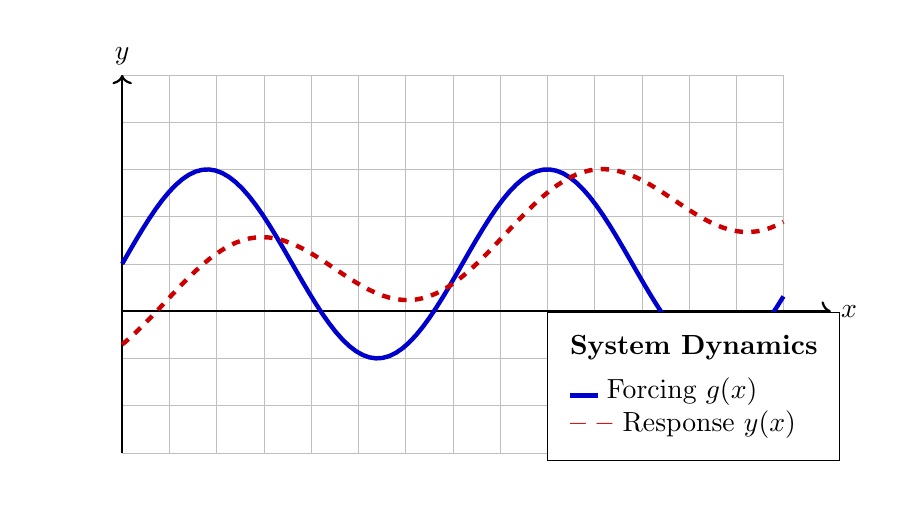
\begin{tikzpicture}[scale=1.2]
    \fill[white] (-1,-2) rectangle (8, 3);
    % Grid
    \draw[lightgray, very thin, step=0.5] (0,-1.5) grid (7,2.5);
    % Axes
    \draw[->, thick] (0,0) -- (7.5,0) node[right] {$x$};
    \draw[->, thick] (0,-1.5) -- (0,2.5) node[above] {$y$};
    
    % Plots
    \draw[ultra thick, blue!80!black, domain=0:7, samples=100] plot (\x, {sin(\x*100) + 0.5});
    \draw[ultra thick, red!80!black, dashed, domain=0:7, samples=100] plot (\x, {0.5*sin(\x*100 - 45) + 0.2*\x});
    
    % Legend using single node and anchor pivot strategy
    \node[align=left, draw, fill=white, inner sep=8pt, anchor=west] at (4.5, -0.8) {
        \textbf{System Dynamics} \\[4pt]
        \textcolor{blue!80!black}{\rule{10pt}{2pt}} Forcing $g(x)$ \\
        \textcolor{red!80!black}{\textbf{-- --}} Response $y(x)$
    };
\end{tikzpicture}
\end{center}

\newpage
\section{Abstract Real-World Modeling (AI, ML, \& Quant Finance)}

\subsection{Concrete Scenarios}
\begin{enumerate}
    \item \textbf{Quantitative Finance (Mean-Reverting Processes with Seasonality):} In algorithmic trading, commodities (like natural gas) often follow a mean-reverting stochastic process (Ornstein-Uhlenbeck) but with a deterministic seasonal forcing term (e.g., higher prices in winter). The expected value of this process is governed by a nonhomogeneous linear ODE, solvable via undetermined coefficients.
    \item \textbf{Machine Learning (Gradient Descent Dynamics):} The continuous-time limit of gradient descent with momentum can be modeled as a second-order damped harmonic oscillator. If the loss landscape has a constant slope in a certain direction (a linear forcing term), the trajectory of the weights follows a nonhomogeneous ODE.
\end{enumerate}

\subsection{Model Problem Setup: Seasonal Commodity Pricing}
Let $X_t$ be the spot price of a seasonal commodity. We model $X_t$ using a modified Ornstein-Uhlenbeck process with a deterministic seasonal mean level $\mu(t)$:
\[
dX_t = \theta(\mu(t) - X_t)dt + \sigma dW_t
\]
where $\theta > 0$ is the speed of mean reversion, $\sigma > 0$ is the volatility, $W_t$ is a standard Brownian motion, and the seasonal mean is modeled as a sinusoid:
\[
\mu(t) = \mu_0 + A \cos(\omega t)
\]
Taking the expectation $\E[\cdot]$ of both sides and letting $y(t) = \E[X_t]$, the stochastic integral vanishes ($\E[dW_t] = 0$), yielding a deterministic first-order linear ODE:
\[
\frac{dy}{dt} = \theta(\mu_0 + A \cos(\omega t) - y) \implies y' + \theta y = \theta \mu_0 + \theta A \cos(\omega t)
\]
This is a nonhomogeneous linear ODE with constant coefficients. The forcing function is $g(t) = \theta \mu_0 + \theta A \cos(\omega t)$.
Using the Annihilator Method, $g(t)$ is annihilated by $D(D^2 + \omega^2)$. The homogeneous root is $r = -\theta$. Since there is no overlap, the form of the particular solution (the steady-state expected price trajectory) is:
\[
y_p(t) = C_1 + C_2 \cos(\omega t) + C_3 \sin(\omega t)
\]
By substituting $y_p(t)$ back into the ODE, a quantitative researcher can exactly solve for the phase shift and amplitude dampening of the expected commodity price relative to the seasonal forcing $\mu(t)$, allowing for precise derivative pricing.

\newpage
\section{Common Variations and Untested Concepts}

\subsection{Variation of Parameters}
The homework exclusively covers the Method of Undetermined Coefficients. However, this method \textbf{fails completely} if $g(x)$ is not a polynomial, exponential, or sinusoid (e.g., $g(x) = \tan x$, $\ln x$, or $\frac{1}{x}$). For these, we must use \textbf{Variation of Parameters}.

\textbf{Concept:} Instead of guessing constant coefficients, we assume the parameters are functions of $x$. If the homogeneous solution is $y_c = c_1 y_1 + c_2 y_2$, we guess:
\[
y_p(x) = u_1(x) y_1(x) + u_2(x) y_2(x)
\]
By substituting this into the ODE and applying constraints, we derive the formulas:
\[
u_1(x) = \int \frac{-y_2(x) g(x)}{W(y_1, y_2)} \, dx, \quad u_2(x) = \int \frac{y_1(x) g(x)}{W(y_1, y_2)} \, dx
\]
where $W(y_1, y_2) = y_1 y_2' - y_1' y_2$ is the Wronskian.

\textbf{Example:} Solve $y'' + y = \sec x$.
1. Homogeneous: $r^2 + 1 = 0 \implies r = \pm i$. So $y_1 = \cos x$, $y_2 = \sin x$.
2. Wronskian: $W(\cos x, \sin x) = (\cos x)(\cos x) - (-\sin x)(\sin x) = \cos^2 x + \sin^2 x = 1$.
3. Apply formulas:
\begin{align*}
u_1(x) &= \int \frac{-\sin x \sec x}{1} \, dx = \int -\tan x \, dx = \ln|\cos x| \\
u_2(x) &= \int \frac{\cos x \sec x}{1} \, dx = \int 1 \, dx = x
\end{align*}
4. Particular Solution: $y_p(x) = (\ln|\cos x|)\cos x + x \sin x$.

\subsection{Euler-Cauchy Equations}
Another variation not tested is linear ODEs with \textit{variable} coefficients of a specific form, such as $x^2 y'' + a x y' + b y = g(x)$. These require a substitution $x = e^t$ to transform them into constant coefficient equations before the annihilator method can be applied.

\newpage
\section{Advanced Diagnostic Testing: "Find the Flaw"}

Below are five problems with complete solutions. Each solution contains a single, subtle, yet critical flaw. Your task as the grader is to find the error, explain it, and correct it.

\vspace{1em}
\textbf{Problem 1:} Find the form of $y_p$ for $y'' - 4y = e^{2x}$.
\begin{itemize}
    \item \textit{Flawed Solution:} The homogeneous equation is $r^2 - 4 = 0$, so $r = \pm 2$. The nonhomogeneous term is $e^{2x}$, which has the annihilator $D-2$. The guess is $y_p = A e^{2x}$.
    \item \textbf{The Flaw:} The student failed to account for root overlap. The root $r=2$ is already in the homogeneous solution.
    \item \textbf{Correction:} Multiply the guess by $x$. The correct form is $y_p = A x e^{2x}$.
\end{itemize}

\vspace{1em}
\textbf{Problem 2:} Find the annihilator for $g(x) = x^2 \sin x$.
\begin{itemize}
    \item \textit{Flawed Solution:} The base function $\sin x$ has roots $\pm i$, so the quadratic factor is $D^2 + 1$. Because it is multiplied by $x^2$, we square the operator. The annihilator is $(D^2 + 1)^2$.
    \item \textbf{The Flaw:} The rule for $x^k$ is to raise the operator to the power of $k+1$, not $k$.
    \item \textbf{Correction:} The multiplicity should be $2+1=3$. The correct annihilator is $(D^2 + 1)^3$.
\end{itemize}

\vspace{1em}
\textbf{Problem 3:} Find the form of $y_p$ for $y'' + 2y' + y = x$.
\begin{itemize}
    \item \textit{Flawed Solution:} The homogeneous roots are $r = -1, -1$. The forcing function is $x$, which is a polynomial of degree 1. Therefore, the guess is $y_p = Ax$.
    \item \textbf{The Flaw:} A polynomial guess must include all lower-degree terms, even if they don't explicitly appear in $g(x)$.
    \item \textbf{Correction:} The correct form is $y_p = Ax + B$.
\end{itemize}

\vspace{1em}
\textbf{Problem 4:} Find the annihilator for $g(x) = \sec x$.
\begin{itemize}
    \item \textit{Flawed Solution:} Since $\sec x = \frac{1}{\cos x}$, and the annihilator for $\cos x$ is $D^2 + 1$, the annihilator for $\sec x$ is $(D^2 + 1)^{-1}$.
    \item \textbf{The Flaw:} The annihilator method only works for linear combinations of polynomials, exponentials, and sines/cosines. There is no finite-order polynomial differential operator that annihilates $\sec x$.
    \item \textbf{Correction:} The annihilator method cannot be used here. Variation of Parameters must be used instead.
\end{itemize}

\vspace{1em}
\textbf{Problem 5:} Find the annihilator for $g(x) = e^x + e^{-x}$.
\begin{itemize}
    \item \textit{Flawed Solution:} The annihilator for $e^x$ is $D-1$. The annihilator for $e^{-x}$ is $D+1$. Therefore, the annihilator for the sum is the sum of the operators: $(D-1) + (D+1) = 2D$.
    \item \textbf{The Flaw:} Annihilators for sums of functions with distinct roots are found by \textit{multiplying} the individual operators, not adding them.
    \item \textbf{Correction:} The correct annihilator is $(D-1)(D+1) = D^2 - 1$.
\end{itemize}

\end{document}